\clearpage
\section{Testkonzept}\label{sec:Testkonzept}
Um die Funktionalität der Teilsysteme sowie das Zusammenspiel aller Teilsysteme zu überprüfen, wird in diesem Abschnitt das Testkonzept definiert. In Abbildung \ref{img:Testplan} sind die Validierungsblöcke aufgelistet. Als Anhaltspunkt dienen die im Kapitel \ref{subsec:Projektziele} erwähnten Ziele. Die verschiedenen Tests müssen während der Realisierung durchgeführt und validiert werden. Zu jedem Test sind die dazugehörigen Spezifikationen erläutert. Falls ein Block nicht das erwartete Resultat aufweist oder ein Pflichtziel nicht erreicht wird, werden allfällige Änderungen vorgenommen.

\begin{figure}[h]
	\centering
	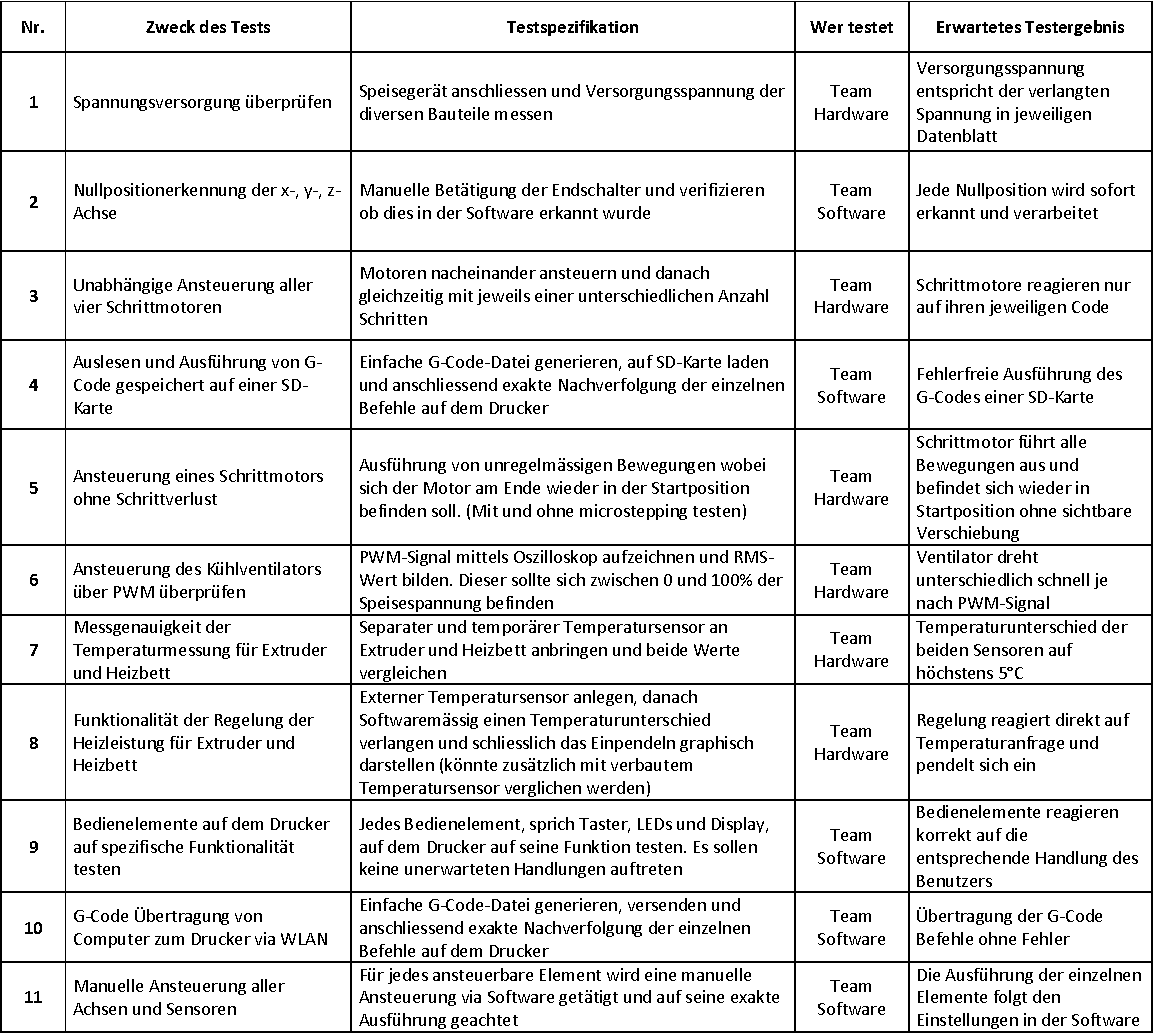
\includegraphics[scale=0.90, angle = 90]{Testplan_Pro4E.pdf}
	\caption{Testkonzept zur Validierung der Projektziele}
	\label{img:Testplan}
\end{figure} 








